\chapter{Fluid Kinematics}
This chapter is based on Munson Chapter 4.

\section{The Velocity Field}

There are two ways of describing a fluid flow, the Eularian, and the Lagrangian approach:
\subsection{Difference Between Eularian and Lagrangian Approach}
For the Eularian approach, we define a velocity field which is a function of the three-dimensional position $\vec r$ and time $t$. From this we know where at which time the stream lines point in a certain direction.

The Lagrangian approach follows particles: A large amount of particles are released and traced as a function of time. 

\begin{figure}[H]
	\centering
	\begin{subfigure}{0.45\textwidth}
		\centering
		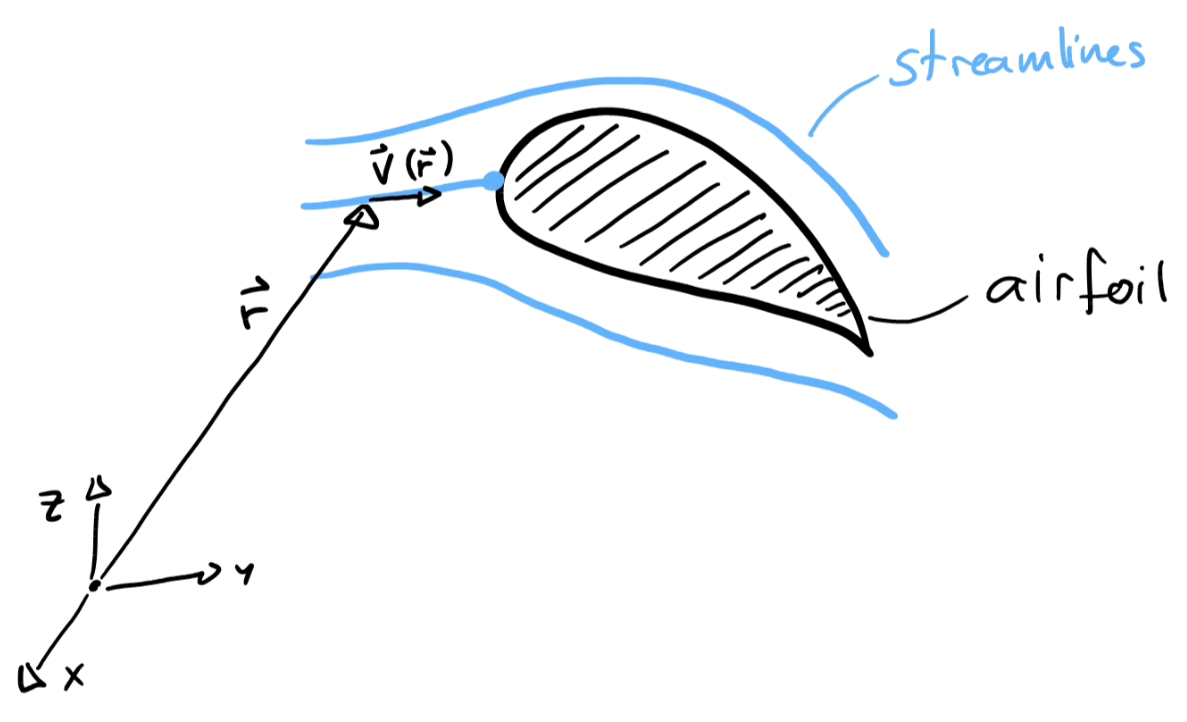
\includegraphics[width=\linewidth]{Sketches/EularianVelocityField}
		\begin{equation*}
			\vec V ( \vec r,t)
		\end{equation*}
		\caption{Eulerian velocity field}
		\label{fig:eularianvelocityfield}
	\end{subfigure}%
	\hfill
	\begin{subfigure}{0.45\textwidth}
		\centering
		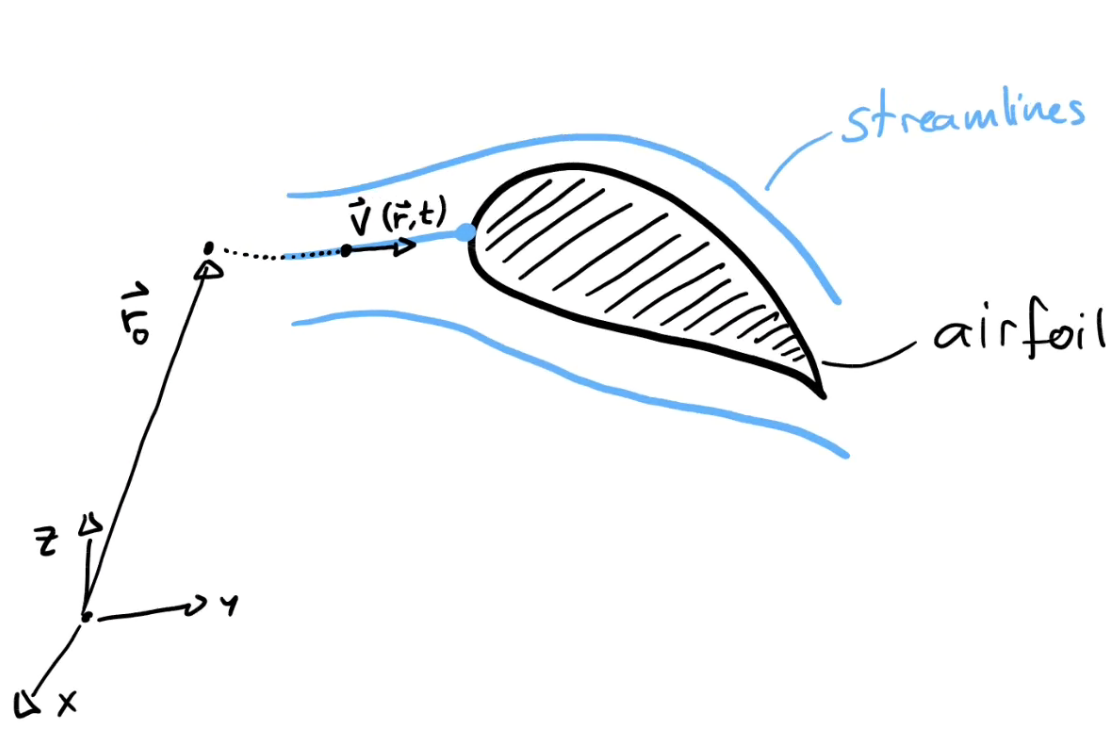
\includegraphics[width=\linewidth]{Sketches/LagrangianVelocityField}
		\begin{equation*}
			\vec V(\vec r_0,t)
		\end{equation*}
		\caption{Lagrangian velocity field}
		\label{fig:lagrangianvelocityfield}
	\end{subfigure}
	\caption{Comparison of (a) Eulerian and (b) Lagrangian velocity field representations}
	\label{fig:velocity_fields}
\end{figure}

\subsection{Visualizing Flows}
\begin{itemize}
	\item \textbf{Stream Line} (\textit{SL}) A line tangent to the velocity vector at any point.

	\begin{figure}[H]
			\centering
			\raisebox{-.5\height}{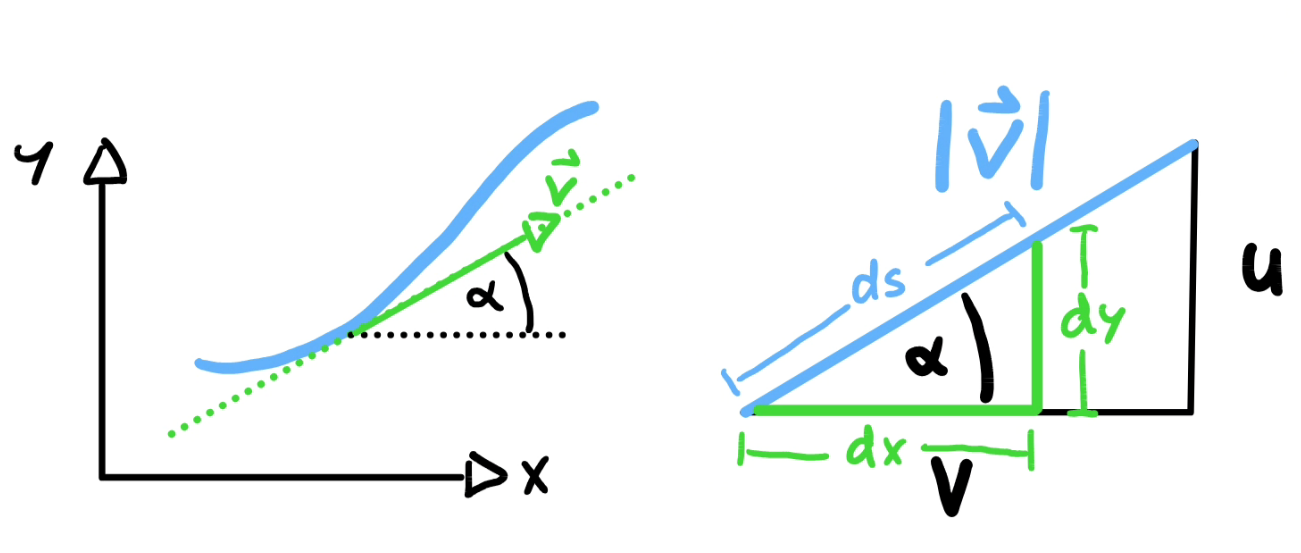
\includegraphics[width=0.4\linewidth]{Sketches/StreamLineEquationDerivation}}
			\label{fig:streamlineequationderivation}
	\end{figure}
	
	\begin{equation*}
		\boxed{\frac{dy}{dx} = \frac vu\qquad \frac{dz}{dx} = \frac wu \qquad \frac{dz}{dy} = \frac wv}
	\end{equation*}
	
	we can define the parametrised curve $\vec r_{sl}(s)$, described by:
	\begin{equation*}
		\frac{d\vec r_{sl}(s)}{ds} \times \vec V (\vec r_sp) = \vec 0
	\end{equation*}
	Stream lines are a purely Eurlarian concept.
	
	\item \textbf{Path Line} Line describing the actual path of a fluid element.

	\begin{equation*}
		\frac{d\vec r_p}{dt} = \vec V (\vec r_p(t))
	\end{equation*}
	where $V$ is the velocity at the instantaneous particle location and $\vec r_p$ is the position of a particle. In components this will result in:
	\begin{equation*}
		\boxed{\frac{dx}{dt} = u\qquad \frac{dy}{dt} =v\qquad \frac{dz}{dt} = w}
	\end{equation*}
	This is meant in a Lagrangian sense: We track a particle and register its position as a function of time.
	
	Similarly, we could write, as a ordinary differential equation:
	\begin{equation*}
		\frac{d\vec r_{pl}}{d t} = \vec V(\vec r_{pl},t)\qquad \text{where } \vec r_{pl} (t=t_0) = \vec r_{p_0}
	\end{equation*}
	
	
	\item \textbf{Steak Line} A line made up of particles, that have previously passed through a common point. It can be reconstructed from path lines: 
	\begin{equation*}
		\frac{d \vec \tau_p}{dt} = V(r_p,t)\qquad\text{width }\vec r_p(t=\tau_p) = \vec r_0\implies \vec r_p (t,\tau_p)
	\end{equation*}
\end{itemize}




\begin{figure}[H]
	\centering
	\begin{subfigure}{0.3\textwidth}	
		\centering
		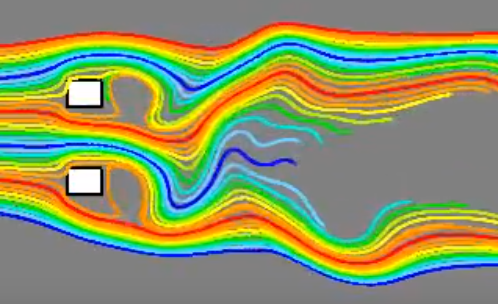
\includegraphics[width=\linewidth]{Sketches/StreamLine}
		\caption{Stream Line}
		\label{fig:streamlines}
	\end{subfigure}
	\hfill
	\begin{subfigure}{0.3\textwidth}
		\centering
		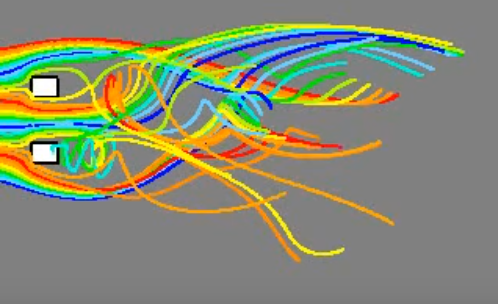
\includegraphics[width=\linewidth]{Sketches/PathLine}
		\caption{Path Line}
		\label{fig:pathline}
	\end{subfigure}%
	\hfill
	\begin{subfigure}{0.3\textwidth}
		\centering
		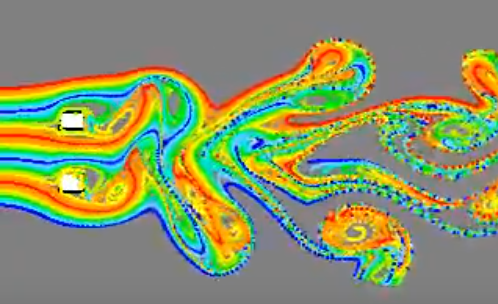
\includegraphics[width=\linewidth]{Sketches/StreakLine}
		\caption{Streak Line}
		\label{fig:streakline}
	\end{subfigure}
	\caption{Comparison of stream, path, and streak line.}
\end{figure}

\subsubsection{Observation}
\begin{center}
	\shadowbox{If the flow is steady, then stream, path and streak lines are identical.}
\end{center}

\subsubsection{Example: Sprinkler (Munson 4.3)}

\begin{figure}[H]
	\centering
	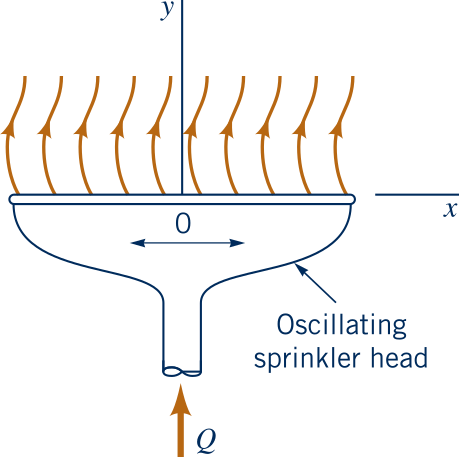
\includegraphics[width=0.45\linewidth]{Sketches/Sprinkler}
	\label{fig:sprinkler}
\end{figure}

let $\omega$ be the oscillation frequency, assume that $x$ and $y$ are infinitely extended. We are given the Eularian velocity field:
\begin{equation*}
	\vec V = U_0\sin\left(\omega \left( t - \frac {y}{v_0}\right)\right)\hat i + v_0 \hat j
\end{equation*}

\paragraph{Stream Line}
From the equation for streamlines we know:
\begin{equation*}
	\begin{split}
		\frac{dy}{dx} &= \frac vu  =\frac{v_0}{U_0\sin\left(\omega \left( t - \frac {y}{v_0}\right)\right)}\\
		U_0 \sin\left(\omega \left( t - \frac {y}{v_0}\right)\right) \,dy & =v_0 \,dx\\
		\int U_0 \sin\left(\omega \left( t - \frac {y}{v_0}\right)\right) \,dy & =\int v_0 \,dx\\ 
		U_0\frac{v_0}{\omega}\cos\left(\omega \left( t - \frac {y}{v_0}\right)\right) & =v_0x + C\\
		\implies x(y) &= \frac{u_0}{\omega}\cos\left(\omega \left( t - \frac {y}{v_0}\right)\right) + C'
	\end{split}
\end{equation*}
We want the stream lines to pass through the origin at $t_0=0$, therefore $C' = \frac {u_0}\omega$:
\begin{equation*}
	x = \frac {u_0}{\omega}\left(\cos\left(\frac{y\omega}{v_0}\right)-1\right)
\end{equation*}
\begin{figure}[H]
	\centering
	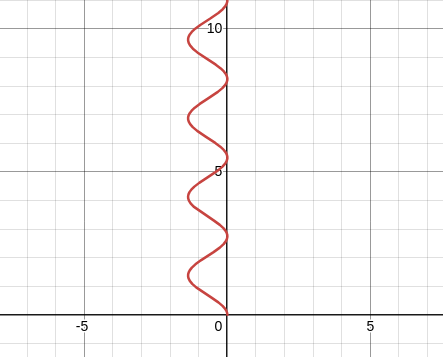
\includegraphics[width=0.4\linewidth]{Sketches/SprinklerStreamLine}
	\caption{Plot of $x(y)$ with $u_0=1.1, \omega= 1.6, v_0=0.7$}
	\label{fig:sprinklerstreamline}
\end{figure}


\paragraph{Path Line}
From the equations of the path line\footnote{in the Lagrangian sense, therefore $y=y(t)$ is the particles position instead of the initial position}, we know:
\begin{equation*}
	\frac{dx}{dt} = U_0 \sin\left(\omega \left( t - \frac {y(t)}{v_0}\right)\right)\qquad \frac{dy}{dt} = v_0
\end{equation*}
We first solve the differential equation for the $y$, yielding:
\begin{equation*}
	y(t) = v_0 t+ c_1
\end{equation*}
plugging this in, we transform the first differential equation into
\begin{equation*}
	\frac{dx}{dt} = U_0 \sin\left(\omega \left( t - \frac {v_0t + c_1}{v_0}\right)\right)=-U_0 \sin\left(\frac {\omega c_1}{v_0}\right)
\end{equation*}
The right hand side are all constants, therefore we can trivially find the solution for $x$:
\begin{equation*}
	x = -U_0\sin\left(\frac{c_1 \omega}{v_0}\right) t + c_2
\end{equation*}

Our parametric equations for path lines are
\begin{equation*}
	\begin{cases}
		x(t) = -U_0\sin\left(\frac{c_1 \omega}{v_0}\right) t + c_2\\
		y(t) = v_0 t+ c_1
	\end{cases}
\end{equation*}
We can represent different particles by varying $c_1$ and $c_2$. For example through algebra, we can find the constants of the particle that is released at $t=0$ at the origin $(x,y)=\vec 0$ to be $c_1=0, c_2=0$.
The path line of this particle is given by:
\begin{equation*}
	\begin{cases}
		x(t) = 0\\
		y(t) = v_0 t
	\end{cases}
\end{equation*}
meaning that it will move along the $y$ axis.


\paragraph{Streak Line}
We choose the streak line that goes though the origin at $t=0$. Knowing that streak lines can be reconstructed from path lines, we try to list all streak lines possible. They will all be linear with slopes varying from $\pm v_0/u_0$. As a streak line we will get something like the following picture:
\begin{figure}[H]
	\centering
	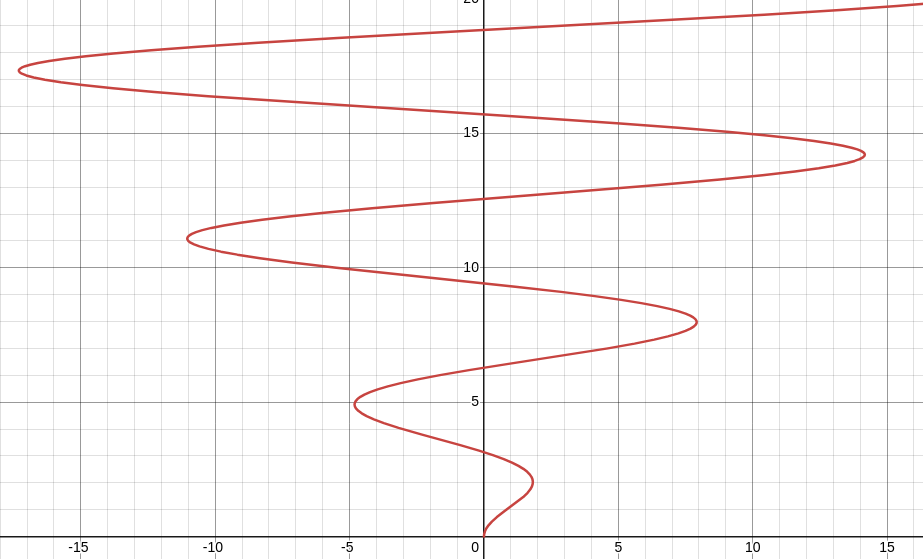
\includegraphics[width=0.4\linewidth]{Sketches/SprinklerStreakLine}
	\label{fig:sprinklerstreakline}
\end{figure}
Which is exactly the droplet pattern that we would observe as a bystander.

\section{Acceleration Field}

In the Lagrangian sense, 
\begin{equation*}
	\vec a = \frac{d\vec V}{dt}=\lim_{\Delta t \to 0}\frac{\vec V(t+\Delta t)-\vec V(t)}{\Delta t}
\end{equation*}

In the Eularian sense\footnote{Note that the acceleration is $\frac{d\vec V}{dt}$, whereas $\frac{\partial \vec V}{\partial t}$ is only par of the acceleration. This is the moment we need to watch out for partial and total derivatives. In fluid dynamics, $\frac{d}{dt} =: \frac{D}{Dt}$ (known as the \enquote{substantial derivative}, \enquote{material derivative}, \enquote{Lagrangian derivative}, or \enquote{derivative following the fluid}) is used to make sure that it is no partial derivative.} ,
\begin{equation*}
	\begin{split}
		\vec a &= \frac{d\vec V(r(t),t)}{dt} = \frac{d\vec V(x(t),y(t),z(t),t)}{dt} \\
		&= 
	\frac{\partial \vec V}{\partial x}\underbrace{\frac{dx}{dt}}_u + 
	\frac{\partial \vec V}{\partial y}\underbrace{\frac{dy}{dt}}_v + 
	\frac{\partial \vec V}{\partial z}\underbrace{\frac{dz}{dt}}_w + 
	\frac{\partial \vec V}{\partial t}\\
	&=(\vec V \cdot \nabla ) \vec V  + \frac{\partial \vec V}{\partial t}
	\end{split}
\end{equation*}
The acceleration field expressed in the eularian velocity field can be therefore expressed as:
\begin{equation*}
	\vec a = \frac{D\vec V}{Dt} = \underbrace{\frac{\partial \vec V}{\partial t}}_{\substack{\text{local}\\\text{acceleration}}} + \underbrace{(\vec V \cdot \nabla)\vec V}_{\substack{\text{convective}\\\text{acceleration}}}
\end{equation*}
If the flow is steady, then \begin{equation*}
	\frac{\partial \vec V}{\partial t} = 0
\end{equation*}

\subsection{Example: Diffuser (Munson Problem 4.31)}

\begin{figure}[H]
	\centering
	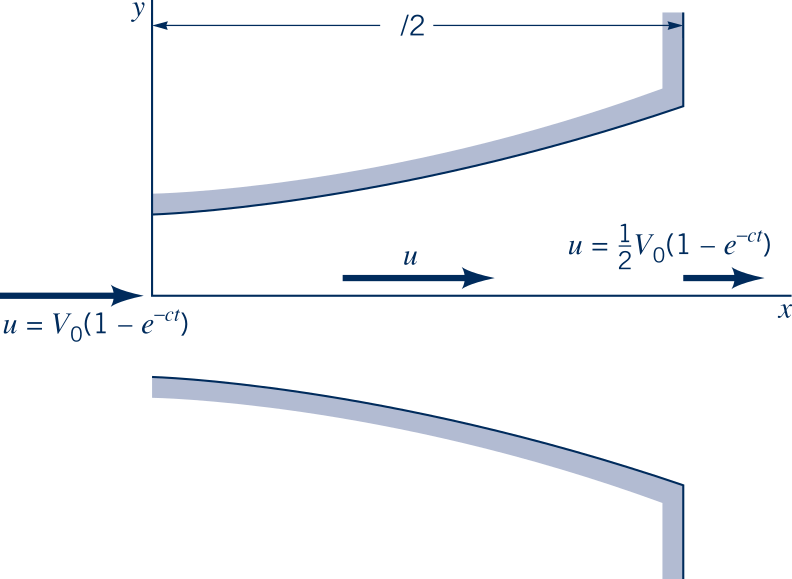
\includegraphics[width=0.4\linewidth]{Sketches/Diffuser}
	\label{fig:diffuser}
\end{figure}
We are given 
\begin{equation*}
	\vec V(x\hat i ,t ) = V_0(1-e^{-ct})\left(1-\frac xl\right)\hat i
\end{equation*}

This leads to a one-dimensional, unsteady differential equation
\begin{equation*}
	\begin{split}
		u(x,t) &= V_0(1-e^{-ct})\left(1-\frac xl\right)\qquad v=w=0\\
		\vec a & = a_x \hat i  = \left(
		\frac{\partial u}{\partial t} + 
		u\frac{\partial u}{\partial x} + 
		v\frac{\partial u}{\partial y} + 
		w\frac{\partial u}{\partial y} + 
		\right)\hat i\\ &= V_0\left(1-\frac xl\right) \left(ce^{-ct}-\frac {V_0}L\left(1-e^{-ct}\right)^2\right)\hat i\\\\
		t\to \infty &\implies\vec V \text{ steady}\\
		& \implies \vec a  =-V_0\left(1-\frac xl\right)\frac {V_0}L\hat i
	\end{split}
\end{equation*}
If we follow the particle, it has a high speed at first, then a slow speed at infinity. The local acceleration goes to zero due to steadiness, but the convective acceleration does not go to zero.

\section{Control Volume and \enquote{System}}
We defined \textit{system} as a collection of matter of fixed identity. For example dyed fluid elements. It has controlled mass. It is a Lagrangian concept, moving with the flow.

The \textit{control volume} is the eularian counterpart: it is a fixed volume in space with a boundary and we observe what goes in and what goes out, though its boundary called \enquote{control surface}.

The physical laws we care about, for example mass conservation is expressed in the Lagrangian concept ($dM/dt = 0$). Rewriting this for a control volume / for eularian concepts intuitively leads us to:
\begin{equation*}
	\left(\frac{dM}{dt}\right)_{cv} = \dot M_{in} - \dot M_{out}
\end{equation*}

What we want to know is the mathematical \enquote{conversion} between the Lagrangian system and Eularian control volume. This method exists and is called \textbf{Reynolds transport theorem}.

\section{Reynolds Transport Theorem (RTT)}

\subsection{Preliminary}
A formal derivation of the Reynolds Transport Theorem can be found in Munson 4.1.1. In this course, we focus on its applications and intuition behind it.

\subsection{Derivation of Simple RTT}


\begin{figure}[H]
	\centering
	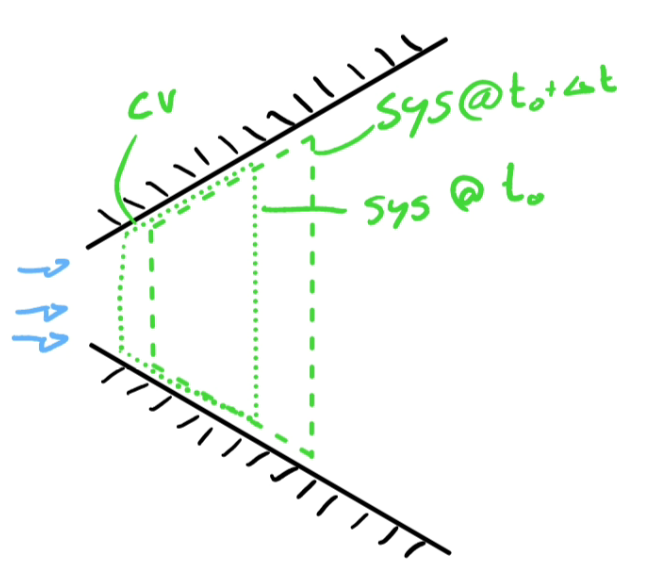
\includegraphics[width=0.4\linewidth]{Sketches/RTTSystemCV}
	\caption{}
	\label{fig:rttsystemcv}
\end{figure}

at $t=t_0$, our system is coincident to the control volume CV ($\mathrm {SYS} =\mathrm{CV}$). $B$ is an extensive quantity (i.e. scaling with the size of the system), and $b = \frac BM$ is an intensive quantity (i.e. independent of the size of the system).

We try to find a total value of $B$ inside the system and control volume in terms of $b$:
\begin{equation*}
	\begin{split}
		B_{sys} &= \int_{sys} \rho b \,dV\\
		B_{cv} &=\int_{cv} \rho b \,dV 
	\end{split}
\end{equation*}

To write the rate of change in the system, we can write
\begin{equation}
	\frac{DB_{sys}}{Dt} = \frac{\partial B_{cv}}{\partial t} + \dot B_{out} - \dot B_{in}
	\label{eq:rtt_rate_of_change}
\end{equation}
where $\dot B_{out,in}$ are the fluxes out and into the control volume. They can be expressed as
\begin{equation*}
	\begin{split}
		\dot B_{in} &= b_{in}\dot M_{in}\stackrel{(*)}{=} b_{in}\rho_{in}v_{in}A_{in}\\
		\dot B_{out} &= b_{out}\dot M_{out}\stackrel{(*)}{=} b_{out}\rho_{out}v_{out}A_{out}\\
	\end{split}
\end{equation*}
At $(*)$ we use $\dot M_{in}=A_{in}\rho v_{in}$. is the product of the input area, density and velocity.

The rate of change of $B$ with the system can be expressed by 
\begin{equation*}
	\boxed{\left(\frac{DB}{Dt}\right)_{sys} = \left(\frac{\partial B}{\partial t}\right)_{cv} + \left(b\rho v A\right)_{out}- \left(b\rho v A\right)_{in}}
\end{equation*}
This is a simple form of the RTT. The simplification we made, was a simplification about the flux term: the \textbf{inlet and outlet areas are flat and their velocities are constant}. To get a general equation, we need to further investigate the flux through the surfaces.

\subsection{General RTT}
The net mass flux though the surface $A$:

\begin{figure}[H]
	\centering
	\begin{subfigure}[b]{0.5\linewidth}
		\centering
		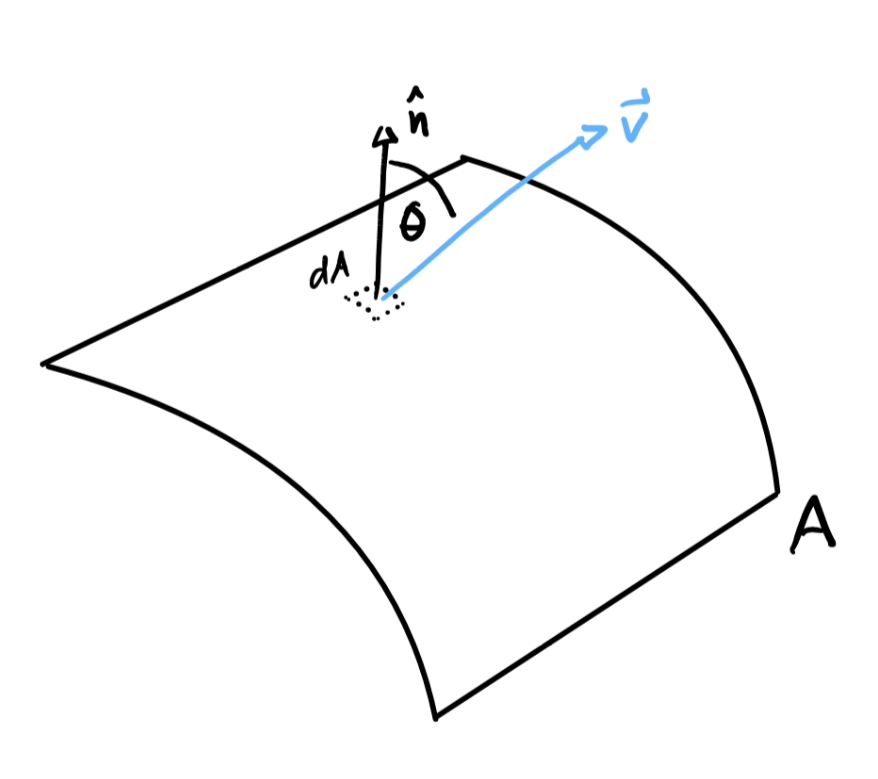
\includegraphics[width=\linewidth]{Sketches/RTTSystemArea}
		\caption{}
		\label{fig:rttsystemarea}
	\end{subfigure}
	\hfill
	\begin{subfigure}[b]{0.3\linewidth}
		\centering
		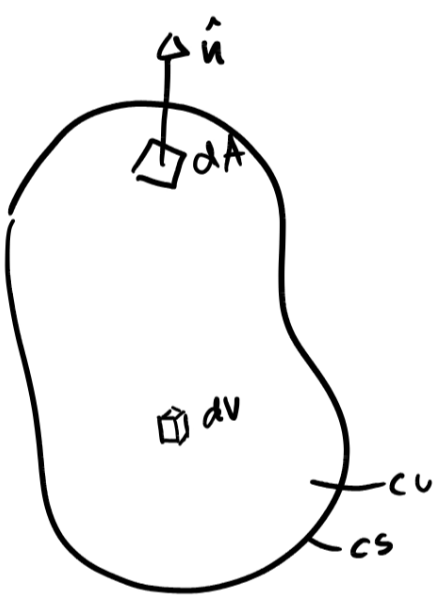
\includegraphics[width=\linewidth]{Sketches/RTTSystemVolume}
		\caption{}
		\label{fig:rttsystemvolume}
	\end{subfigure}
	\caption{}
	\label{fig:rttsystem}
\end{figure}

is expressed as 
\begin{equation*}
	\dot M = \int_A \rho \underbrace{v\cos\theta}_{\substack{\text{normal}\\\text{component}}} \,dA\implies \dot B = \int_A b\rho \vec v \cdot \hat n \,dA = \dot B_{out} - \dot B_{in}
\end{equation*}
where $\dot B$ is the net flux.

This allows us to rewrite eq. \eqref{eq:rtt_rate_of_change} as:
\begin{equation}
	\boxed{\left(\frac{DB}{Dt}\right)_{sys} = \frac{\partial}{\partial t}\int_{cv} \rho b \,dV + \int_{cs} \rho b \vec v \cdot \hat n \,dA}
	\label{eq:rtt_final}
\end{equation}
Which is the equation we can use to transform a system from the Eularian to the Lagrangian point of view and vice versa.
\subsection{Notes}
For a steady flow, the first integral in \eqref{eq:rtt_final} vanishes as it is not time dependant.

\begin{equation*}
	\left(\frac{DB}{Dt}\right)_{sys} = \int_{cs} \rho b \vec v \cdot \hat n \,dA 
\end{equation*}


A moving, but non-deforming (!!) control volume, we can use relative velocities:
\begin{equation*}
	\vec w = \vec v - \vec v_{cv}
\end{equation*}

If we integrate over a closed surface:
\begin{equation*}
	 \oint_{cs} \rho b \vec v \cdot \hat n \,dA 
\end{equation*}
we can often split it up










